\documentclass[11pt,a4paper]{article}
\usepackage[margin=18mm,headheight=24pt]{geometry}
\usepackage[T1]{fontenc}
\usepackage[english]{babel}
\usepackage{lmodern}
\usepackage{microtype}
\usepackage{amsmath,amssymb}
\usepackage{siunitx}
\usepackage{tikz}
\usetikzlibrary{arrows.meta,calc,angles,quotes}
\usepackage{enumitem}
\usepackage{xcolor}
\usepackage{fancyhdr}
\usepackage{lastpage}
\usepackage[hidelinks]{hyperref}

\definecolor{VectorGreen}{HTML}{174A38}
\definecolor{VectorAccent}{HTML}{216343}
\definecolor{VectorMint}{HTML}{E2F0E5}
\definecolor{VectorCoral}{HTML}{C45136}
\definecolor{VectorInk}{HTML}{203B31}
\definecolor{VectorMuted}{HTML}{5F7468}

\color{VectorInk}
\setlength{\parindent}{0pt}
\setlength{\parskip}{0.55em}
\setlist[enumerate]{leftmargin=*,itemsep=0.45em,topsep=0.35em}
\sisetup{per-mode=symbol}

\pagestyle{fancy}
\fancyhf{}
\lhead{\textcolor{VectorMuted}{Vectors · Exercise session}}
\rhead{\textcolor{VectorMuted}{Addition and subtraction}}
\cfoot{\textcolor{VectorMuted}{\thepage\ / \pageref*{LastPage}}}
\renewcommand{\headrulewidth}{0.4pt}
\renewcommand{\headrule}{\hbox to\headwidth{\color{VectorMint}\leaders\hrule height \headrulewidth\hfill}}

\newcommand{\sessiontitle}[2]{%
  {\color{VectorGreen}\fontsize{25}{29}\selectfont\bfseries #1\par}
  \vspace{0.2em}
  {\color{VectorMuted}\large #2\par}
  \vspace{0.55em}
  {\color{VectorAccent}\rule{\textwidth}{1.5pt}}
}

\newcommand{\problemheading}[2]{%
  {\color{VectorAccent}\small\bfseries\MakeUppercase{Problem #1}}\par
  {\color{VectorGreen}\LARGE\bfseries #2}\par
  \vspace{0.25em}
}

\newcommand{\prediction}[1]{%
  \begin{center}
  \colorbox{VectorMint}{\parbox{0.92\linewidth}{\textbf{Predict before calculating.} #1}}
  \end{center}
}

\newcommand{\checkpoint}[1]{%
  \begin{center}
  \fcolorbox{VectorAccent}{white}{\parbox{0.91\linewidth}{\textbf{Reasoning checkpoint.} #1}}
  \end{center}
}

\newcommand{\worklines}[1]{%
  \par\vspace{0.25em}
  {\color{VectorMuted}\small\textit{Working and explanation}}\par
  \foreach \n in {1,...,#1}{\vspace{0.54cm}\noindent\textcolor{VectorMint}{\rule{\linewidth}{0.35pt}}\par}
}

\newcommand{\answerbox}[1]{%
  \begin{center}
  \colorbox{VectorMint}{\parbox{0.92\linewidth}{\textbf{Answer.} #1}}
  \end{center}
}


\begin{document}

\sessiontitle{Vectors that fool intuition}{Four problems about what vector addition and subtraction really mean}


\vspace{0.55em}
For every problem, make a prediction, draw the relevant arrows, calculate, and explain the physical meaning of the result. Use east as $+x$ and north as $+y$ unless stated otherwise.


\problemheading{1}{Same sum. Same journey?}

Aruzhan and Daniyar start at the origin at the same time. Each walks at a constant speed of \SI{1}{m/s} and turns instantly at the corner.

\begin{itemize}[leftmargin=*,itemsep=0.25em]
  \item Aruzhan walks \SI{3}{m} east, then \SI{4}{m} north.
  \item Daniyar walks \SI{4}{m} north, then \SI{3}{m} east.
\end{itemize}

\prediction{Because $\vec a+\vec b=\vec b+\vec a$, must they be at the same place at every time?}

\begin{center}
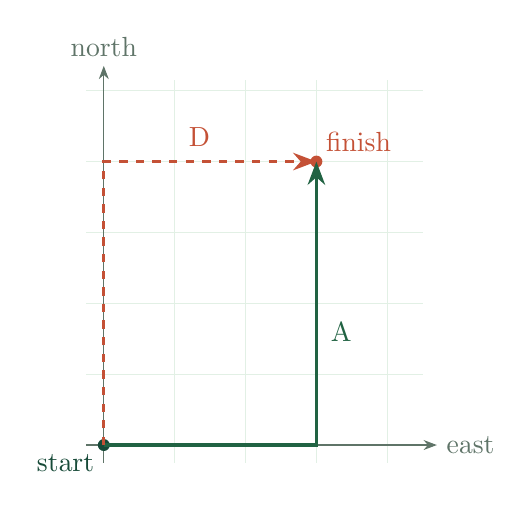
\begin{tikzpicture}[>=Stealth,scale=0.9]
  \draw[step=1cm,VectorMint,thin] (-0.25,-0.25) grid (4.5,5.15);
  \draw[->,VectorMuted] (-0.25,0) -- (4.7,0) node[right] {east};
  \draw[->,VectorMuted] (0,-0.25) -- (0,5.35) node[above] {north};
  \fill[VectorGreen] (0,0) circle (2.4pt) node[below left] {start};
  \fill[VectorCoral] (3,4) circle (2.4pt) node[above right] {finish};
  \draw[->,very thick,VectorAccent] (0,0) -- (3,0) -- (3,4);
  \draw[->,very thick,VectorCoral,dashed] (0,0) -- (0,4) -- (3,4);
  \node[VectorAccent] at (3.35,1.6) {A};
  \node[VectorCoral] at (1.35,4.35) {D};
\end{tikzpicture}
\end{center}

\begin{enumerate}[label=\alph*)]
  \item Find each person's final position, displacement, distance travelled, average velocity, and average speed.
  \item Apart from the start, determine exactly when they occupy the same position. Show how you know.
  \item At $t=\SI{3.5}{s}$, find both position vectors and the vector from Aruzhan to Daniyar.
  \item State precisely what the commutative law guarantees here—and what it does not guarantee.
\end{enumerate}

\worklines{6}


\problemheading{2}{Two apps disagree—or do they?}

A drone makes one displacement. App E uses east and north as its positive axes and reports
\[
  (3,4)\ \si{km}.
\]
App N uses north and west as its positive axes and reports
\[
  (4,-3)\ \si{km}.
\]

\prediction{Do the two ordered pairs represent different displacements? Should they be added?}

\begin{center}
\begin{tikzpicture}[>=Stealth,scale=1.05]
  \coordinate (O) at (0,0);
  \draw[->,VectorAccent,thick] (O) -- (4.2,0) node[right] {$+x_E$: east};
  \draw[->,VectorAccent,thick] (O) -- (0,4.7) node[above] {$+y_E$: north};
  \draw[->,VectorCoral,thick] (O) -- (0,3.6) node[left] {$+x_N$: north};
  \draw[->,VectorCoral,thick] (O) -- (-3.6,0) node[left] {$+y_N$: west};
  \draw[->,very thick,VectorGreen] (O) -- (3,4) node[above right] {$\vec d$};
  \draw[dashed,VectorMuted] (3,0) -- (3,4) -- (0,4);
  \node[below left] at (O) {start};
\end{tikzpicture}
\end{center}

\begin{enumerate}[label=\alph*)]
  \item Use the diagram to explain every number and sign in both reports.
  \item Convert App N's pair into App E's east--north coordinates.
  \item A student calculates $(3,4)+(4,-3)=(7,1)$. Identify the exact mathematical error.
  \item Another student subtracts the reports. What should the difference of the two physical displacement vectors be? Show the valid calculation.
  \item Write one rule that must be followed before adding or subtracting component pairs.
\end{enumerate}

\worklines{6}


\problemheading{3}{Equal speeds on a collision course}

Two drones fly at constant velocity. At $t=0$, their positions and velocities are
\[
\vec r_A=(0,0)\ \si{m},\qquad \vec v_A=(4,0)\ \si{m/s},
\]
\[
\vec r_B=(8,-8)\ \si{m},\qquad \vec v_B=(0,4)\ \si{m/s}.
\]
Thus both drones have the same speed, \SI{4}{m/s}, but they fly in perpendicular directions.

\prediction{Will they collide? A comparison of their speeds alone is not enough—make a position sketch.}

\begin{center}
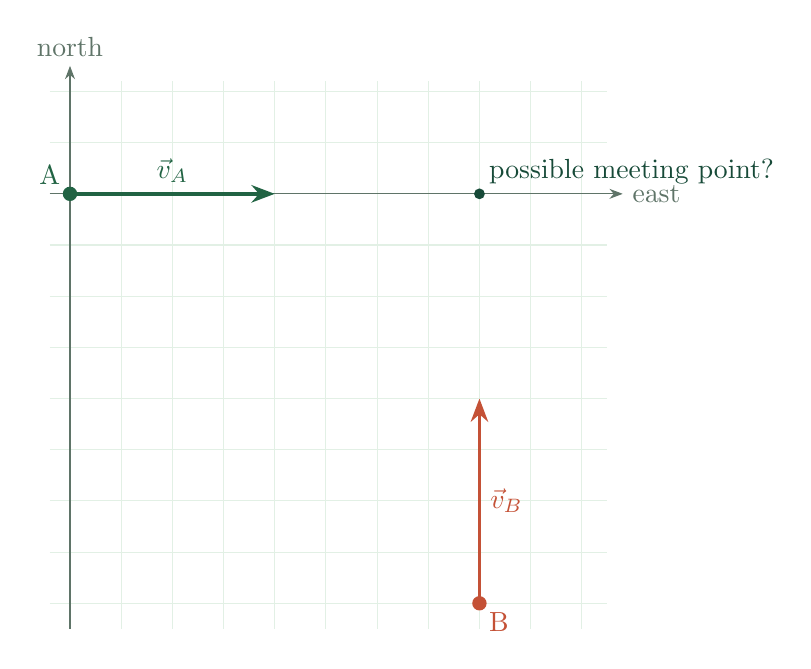
\begin{tikzpicture}[>=Stealth,scale=0.65]
  \draw[step=1cm,VectorMint,thin] (-0.4,-8.5) grid (10.5,2.2);
  \draw[->,VectorMuted] (-0.4,0) -- (10.8,0) node[right] {east};
  \draw[->,VectorMuted] (0,-8.5) -- (0,2.5) node[above] {north};
  \fill[VectorAccent] (0,0) circle (4pt) node[above left] {A};
  \draw[->,very thick,VectorAccent] (0,0) -- (4,0) node[midway,above] {$\vec v_A$};
  \fill[VectorCoral] (8,-8) circle (4pt) node[below right] {B};
  \draw[->,very thick,VectorCoral] (8,-8) -- (8,-4) node[midway,right] {$\vec v_B$};
  \fill[VectorGreen] (8,0) circle (3pt) node[above right] {possible meeting point?};
\end{tikzpicture}
\end{center}

\begin{enumerate}[label=\alph*)]
  \item Find B's initial position relative to A: $\vec r_{B/A}=\vec r_B-\vec r_A$.
  \item Find B's velocity relative to A: $\vec v_{B/A}=\vec v_B-\vec v_A$. Draw it.
  \item Use $\vec r_{B/A}(t)=\vec r_{B/A}(0)+\vec v_{B/A}t$ to decide whether they collide. If they do, find the time and place.
  \item Explain why ``their speeds are equal, so neither catches the other'' is faulty reasoning.
\end{enumerate}

\worklines{5}

\end{document}
